	\documentclass[10pt,oneside]{CBFT_book}
	% Algunos paquetes
	\usepackage{amssymb}
	\usepackage{amsmath}
	\usepackage{graphicx}
	\usepackage{libertine}
% 	\usepackage[bold-style=TeX]{unicode-math}
	\usepackage{lipsum}

	\usepackage{natbib}
	\setcitestyle{square}

	\usepackage{polyglossia}
	\setdefaultlanguage{spanish}


	\usepackage{CBFT.estilo} % Cargo la hoja de estilo
	
	% Tipografías
	% \setromanfont[Mapping=tex-text]{Linux Libertine O}
	% \setsansfont[Mapping=tex-text]{DejaVu Sans}
	% \setmonofont[Mapping=tex-text]{DejaVu Sans Mono}

	%===================================================================
	%	DOCUMENTO PROPIAMENTE DICHO
	%===================================================================

% \title{CBFT Mecánica clásica}
% \author{Fuerzas centrales}
% \date{\today}

\begin{document}
% \maketitle
% \tableofcontents

\chapter{Fuerzas centrales}

% =================================================================================================
\section{Fuerzas centrales}\index{Fuerzas centrales}
% =================================================================================================

\notamargen{Comentario de que fijo un punto, y es una función vectorial tomar vector y da vector, que resulta finalmente
más simple porque se sabe de antemano la dirección de la salida --en la dirección de la recta que une los puntos--.}

Una fuerza central es aquella que depende únicamente de la distancia entre dos puntos. Es decir que si se tienen dos
puntos $\vb{x}, \vb{y}$, separados una distancia $ r = |\vb{r}| = |\vb{x} - \vb{y}| $, una fuerza central $\vb{F}$ verifica
\[
	\vb{F}( \vb{x}, \vb{y} ) = F(r) \: \hat{r}, \qquad \qquad \hat{r} = \frac{\vb{r}}{r}
\]
% es decir que la fuerza $\vb{F}$ entre dos puntos $\vb{x}, \vb{y}$ depende de la distancia $r = |\vb{x}-\vb{y}|$
% entre los mismos.
de manera que la información sobre la dirección de la misma ($\hat{r}$) está establecida en la recta que une $\vb{x}$ con 
$\vb{y}$ mientras que su módulo es una función escalar $F(r)$.


\begin{figure}[!hbt]
	\begin{center}
	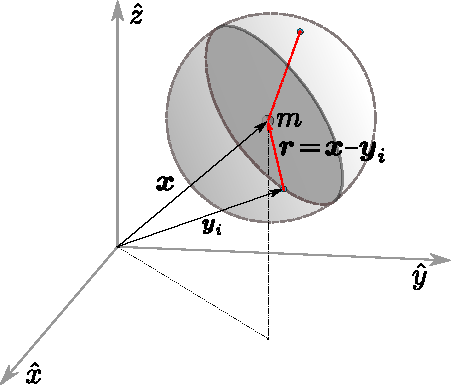
\includegraphics[width=0.4\textwidth]{images/fig_fuerza_central.pdf}	 
	\end{center}
	\caption{}
\end{figure} 

Esto implica, al ser una fuerza dependiente de una sola coordenada, que siempre es posible obtener un potencial
a partir de ella, es decir que existe $V(r)$ tal que
\[
	F(r) = - \dpar{V}{r}.
\]
\notamargen{Hay que elaborar bastante aquí: la fuerza central implica la simetría esférica porque tomado como origen
de coordenadas uno de los dos puntos $\vb{x}$ o $\vb{y}$, la fuerza por otro punto que se halle a la misma distancia
$r$ tendrá la misma magnitud. Además, el torque de la fuerza respecto a ese origen será nulo puesto que son paralelos
$\vb{r}$ y $\vb{F}$. Anoté en la carpeta: el lagrangiano es un potencial de superficies equipotenciales esféricas, entonces
se conserva el momento angular.}

Entonces, para una partícula libre el lagrangiano se puede escribir en coordenadas esféricas $(r,\theta,\phi)$ como
\[
	\Lag = \frac{1}{2}m \left( \dot{r}^2 + r^2 \dot{\theta}^2 + r^2 \sin(\theta)^2\dot{\phi}^2 \right)
\]

El momento angular $\vb{L}$ se conserva puesto que $\vb{\tau} = \vb{x} \times \vb{F}=0$. Como es 
$\vb{L} = \vb{x} \times \vb{p} = \vb{x} \times m \: \dot{\vb{x}} = cte$ entonces se sigue que $\vb{r},\vb{p}$
se hallan contenidos en el mismo plano.

Puedo pedir, sin pérdida de generalidad, que $\theta=\pi/2$ (se sitúa la partícula en el plano $xy$) y entonces
se tienen dos grados de libertad,
\[
	\Lag = \frac{1}{2}m \left( \dot{r}^2 + r^2 \dot{\theta}^2 \right) - V(r).
\]

Como $\phi$ es cíclica se tiene
\be
	\dpar{\Lag}{\dot{\phi}} = L = mr^2\dot{\phi}
	\label{ec_mov_uno}
\ee
que no es otra cosa que la conservación del momento angular (la primera ecuación de movimiento). Esa información puede 
ser llevada al lagrangiano,
\be
	\Lag = \frac{1}{2}m \dot{r}^2 + \left[ \frac{L^2}{2 m r^2} - V(r) \right]
	\label{lag_pot_central}
\ee
donde el último corchete será lo que llamaremos un potencial efectivo\footnote{Debido a la conservación del momento 
angular la parte de la energía dependiente de $\phi$, o mejor dicho debida a la rotación en $\phi$ se ha podido 
expresar en términos de $r$; entonces pasa a formar parte del potencial.}\index{potencial efectivo} $V_{\text{eff}}$, y 
el lagrangiano adopta la forma
\[
	\Lag = \frac{1}{2}m \dot{r}^2 + V_{\text{eff}}(r).
\]
Digamos que el potencial efectivo sería todos aquellos términos que no tienen la forma de la energía cinética 
(cuadrática en velocidades).
Notemos que ahora el lagrangiano depende solamente de $r$; el problema ha resulado para un único grado de libertad.

Dado el sistema elegido (movimiento plano en $xy$) ahora el $p_\phi$ es el $L$ total; en cambio, de haber elegido otro 
plano el $p_\phi$ sería el $L_z$.

La ecuación de Euler-Lagrange para el lagrangiano \eqref{lag_pot_central} resulta en
\[
	m\ddot{r} - \frac{L^2}{mr^3} + \dpar{V}{r} = 0.
\]
Integrando esta ecuación se llega a la conservación de la energía pero podemos utilizar el hecho de saber que la 
misma se conserva y escribir su expresión explícita
\be
	E = T - V = \frac{1}{2}m \dot{r}^2 + \frac{L^2}{2 m r^2} + V(r).
	\label{ec_mov_dos}
\ee

A partir de estas constantes $L,E$ tengo dos ecuaciones de primer orden \eqref{ec_mov_uno} y \eqref{ec_mov_dos}. Se han 
podido {\it ahorrar} dos integraciones: la integral de $\ddot{r}$ para obtener $\dot{r}$ y la integral de $\ddot{\phi}$ 
para hallar $\dot{\phi}$.

Desde la ecuación \eqref{ec_mov_dos} se puede integrar directamente la trayectoria $r=r(t)$ según
\[
	\dtot{r}{t} = \sqrt{ \frac{2}{m}\left( E - \frac{L^2}{2 m r^2} - V(r) \right)},
\]
o bien 
\[
	\int_{t_i}^{t_f} dt = \int_{r(t_i)}^{r(t_f)} \frac{dr}{\sqrt{\frac 2 m ( E - \frac{L^2}{2 m r^2} - V(r) )}},
\]
integral que en principio siempre tiene solución.
A partir de la ecuación \eqref{ec_mov_uno} se puede obtener la trayectoria en el espacio físico $r=r(\phi)$, o 
equivalentemente $\phi=\phi(r)$.
\[
	\dtot{\phi}{t} = \dtot{\phi}{r} \dot{r} =  \frac{L}{mr^2} 
\]
e incorporando de la \eqref{ec_mov_dos} la expresión de $\dot{r}$ se puede llegar a 
\[
	\int_{\phi_i}^{\phi_f} d\phi = \int_{r(\phi_i)}^{r(\phi_f)} 
	\frac{L}{\sqrt{ 2 m r^4 \left( E - \frac{L^2}{2 m r^2} - V(r) \right)}}dr
\]
y la resolución total del problema dependerá de la forma $V(r)$.
\notamargen{Embellecer un poco las expresiones por el aspecto odd de las raíces y todo eso.}

Consideremos, para fijar ideas, un potencial general del tipo 
\[
	V(r)  = \alpha r^{-n} 
\]
que es un potencial cuyo comportamiento dependerá del signo de la constante que acompaña. Los casos posibles serán 
\[
	\alpha = \begin{cases}
	\alpha > 0 \qquad \text{ potencial repulsivo} \\
	\alpha = 0 \qquad \text{ partícula libre} \\
	\alpha > 0 \qquad \text{ potencial repulsivo} 
	\end{cases}
\]
En un gŕafico de potencial y energía en función del radio se pueden analizar muchos aspectos de la física bajo ese 
potencial (como se hizo en el ejemplo XX del capítulo XX)

Para el caso de $\alpha > 0$ se tiene una situación como la que se ilustra en la figura bajo estas líneas
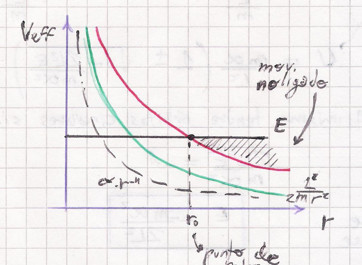
\includegraphics[width=0.4\textwidth]{images/fig_mc_potencialcentral1.jpg}

En el caso de partícula libre, $\alpha=0$, a cierta velocidad se tendrá el siguiente gráfico de potencial. El otro 
gráfico ilustra la posible situación real (en el espacio físico)
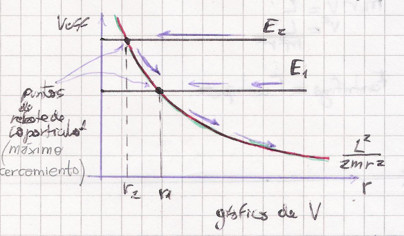
\includegraphics[width=0.4\textwidth]{images/fig_mc_potencialcentral2.jpg}
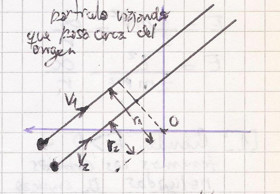
\includegraphics[width=0.4\textwidth]{images/fig_mc_potencialcentral3.jpg}

Finalmente el caso de un potencial atractivo, $\alpha < 0 $ se tienen energias para las cuales el movimiento es ligado.
Cuando existen radios mínimo y máximo se tendrá una órbita como la que se ilustra en el segundo gráfico

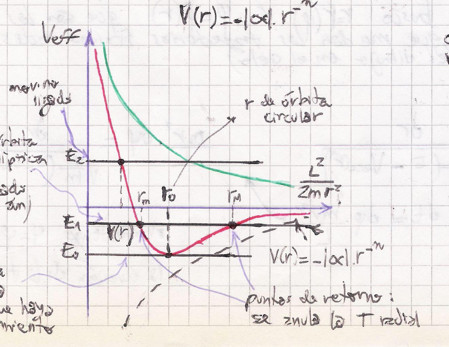
\includegraphics[width=0.4\textwidth]{images/fig_mc_potencialcentral4.jpg}
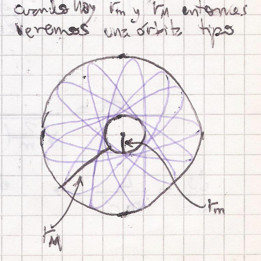
\includegraphics[width=0.4\textwidth]{images/fig_mc_potencialcentral5.jpg}

En los puntos de retorno se anula la energía cinética radial $T$.
El momento angular $L$ es el responsable de que haya satélites orbitando a los planetas; si $L=0$ la partícula pasaría 
por el origen.

En el gráfico bajo estas líneas ilustramos muchas de las características de la física del problema
de fuerzas centrales.

\begin{figure}[!hbt]
	\begin{center}
	\includegraphics[width=0.9\textwidth]{images/fig_mc_potencialcentral.pdf}	 
	\end{center}
	\caption{}
\end{figure} 

\notamargen{Este gráfico hay que tirarlo de inmediato.}

Calculemos ahora los puntos de retorno.
Tomando el cambio de variables $U=1/r$ en la ecuación de la energía es
\[
	\frac{L^2}{2m} U^2 - \alpha U - E = 0,
\]
una cuadrática para $U$ con soluciones
\be
	U = \frac{m\alpha}{L^2}\left( 1 \pm \sqrt{1 + 2L^2E/(m\alpha^2) }\right)
	\label{ec_puntos_retorno_U}
\ee
y entonces
\[
	U_+ = \frac{1}{r_m} \qquad U_- = \frac{1}{r_M}
\]

Si requiereo que $U>0$ en cada caso, necesito $ \sqrt{1 + 2L^2E/(m\alpha^2) } < 1 $ de manera que $ E < 0 $.

Asimismo tendré órbitas circulares si
\[
	\frac{ 2 L^2 E }{ m \alpha^2 } = - 1
\]
lo que significa que 
\[
	E = -\frac{m\alpha^2}{2L^2}.
\]

Puedo calcular el radio de órbita circular haciendco que la fuerza radial se compense exactamente con la fuerza 
centrífuga
\[
	m r v = L
\]
y entonces
\[
	E = \frac{L^2}{2mr^2} - \frac{\alpha}{r}.
\]

Cuando $E>0$ se ve en \eqref{ec_puntos_retorno_U} que se obtienen las órbitas no ligadas; $U_-$ empieza a ser negativa 
y hay que descartarla porque significa un $r_M$ negativo.

Una vez en posesión de $r(t), \phi(t)$ se pueden calcular $r(\phi)$ o $\phi(r)$ que son las funciones que me darán las
trayectorias físicas reales ({\it el dibujo en el cielo}).
Utilizando $d\phi/dt = L/(m r^2 )$ en $dr/dt$ se llega a 
\[
	dt = \frac{dr}{\sqrt{2/m(E-V_{\text{eff}}(r))}}  = \frac{ m r^2 }{ L } d\phi
\]
y ahora se tiene $\phi = \phi(r)$ que es la ecuación de la trayectoria, cuya integral es
\be
	\int_{\phi_0}^{\phi} d\phi = \int_{r_0}^r \frac{L}{mr^2} \frac{dr}{\sqrt{2/m(E-V_{\text{eff}}(r))}}
	\label{integral_trayectoria}
\ee

La ecuación de movimiento para $r$ [¿?]
\[
	m \dtot[2]{r}{t} - \frac{L^2}{mr^3} = -\dtot{V}{r}
\]
y la relación 
\[
	\frac{mr^2}{L} d\phi = dt
\]
permite transformar una derivada temporal en una derivada con respecto al ángulo,
\[
	\dtot{}{t}\left( \phantom{\frac{}{}} \right) = \frac{L}{mr^2} \dtot{}{\phi}\left( \phantom{\frac{}{}} \right)
\]
de modo que la ecuación de arriba se convierte en
\[
	\frac{L}{r^2}\dtot{}{\phi}\left( \frac{L}{mr^2} \dtot{r}{\phi} \right) - \frac{L^2}{mr^3} = -\dtot{V}{r},
\]
es decir en
\[
	-\frac{L^2}{mr^4}\dtot[2]{r}{\phi} - \frac{L^2}{mr^3} = -\dtot{V}{r}.
\]

Proponiendo el cambio de variables $U = 1/r$ se tiene 
\[
	dU = -\frac{1}{r^2} dr,
\]
y entonces
\[
	\dtot{U}{\phi} = -\frac{1}{r^2} \dtot{r}{\phi}.
\]
La ecuación en términos de $U$ luce como
\be
	\dtot[2]{U}{\phi} + U = -\frac{m}{L^2U^2} \: F(1/U),
	\label{ec_fuerza_central_U}
\ee
donde $F(1/U) = dV / dr(U)$.
\notamargen{Esto ilustra un procedimiento elemental y usual en resolución de ecuaciones diferenciales que es el de
cambio de variables. Decir algo al respecto.}

Para el caso de un potencial newtoniano (problema de Kepler) tendremos 
\[
	-\frac{m}{L^2U^2} \: F(1/U) = \frac{\alpha m}{L^2}.
\]

La integral de la trayectoria \eqref{integral_trayectoria} será {\it fea o no} dependiendo de la forma del potencial $V$.
En la ecuación \eqref{ec_fuerza_central_U} tiene una propiedad de simetría puesto que es invariante ante el cambio 
$\vp \to -\vp$. Entonces si utilizamos condiciones de contorno que tengan esta simetría sabremos que la órbita por
encima de $x$ (ver figuretta) es igual a la órbita por debajo.

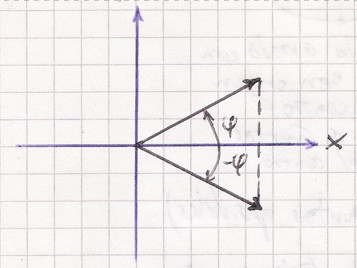
\includegraphics[scale=0.3]{images/fig_mc_orbitas_simetria.jpg}

Las condiciones iniciales 
\[
	\left.\dtot{U}{\vp}\right|_{\vp=0} = U_0' = 0 \qquad \left. U \right|_{\vp=0} = U_0
\]
donde en la condición de la derivada vemos que con la nulidad vale para $\vp$ y para $-\vp$.
Luego, $U_0$ corresponderá a un máximo o mínimo necesariamente porque hacia un lado y hacia otro tengo el mismo
comportamiento.

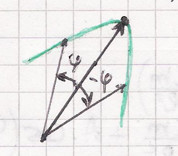
\includegraphics[scale=0.3]{images/fig_mc_orbitas_simetria_2.jpg}

Entonces máximo y mínimo son puntos apsidales, si elijo el eje $x$ ahí tengo simetría de reflexión de la órbita.

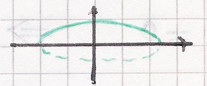
\includegraphics[scale=0.3]{images/fig_mc_orbitas_simetria_3.jpg}
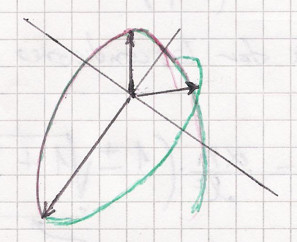
\includegraphics[scale=0.3]{images/fig_mc_orbitas_simetria_4.jpg}

Entonces la integral \eqref{integral_trayectoria} se puede escribir 
\be
	\Delta \vp = 2 \int_{r_{\text{min}}}^{r_{\text{max}}} \frac{L}{2mr^2} \frac{dr}{\sqrt{ 2/m (E - V_{\text{eff}}(r) ) }}
	\label{integral_trayectoria_vp}
\ee
donde $\Delta\vp$[?] es el ángulo que avanza en una oscilación (esto es el ángulo de una oscilación completa).

Si esto es un múltiplo racional de $\pi$ entonces se cierra la órbita; es decir que se tiene la siguiente 
condición de órbita cerrada
\[
	\frac{2\pi}{\Delta \vp} = \frac{m}{n}
\]
donde $m,n$ son enteros.

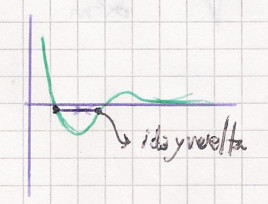
\includegraphics[scale=0.3]{images/fig_mc_orbitas_simetria_5.jpg}

\notamargen{Recordar que problema ligado no implica órbita cerrada.}

Como la integral \eqref{integral_trayectoria_vp} depende de $L, E$ en general tendremos para el problema genérico órbitas
abiertas.

Hay dos problemas que dan órbitas cerradas siempre: son los potenciales 
\[
	V = -\frac{k}{r} \; \text{ \scriptsize{(Problema de Kepler)} } \qquad \qquad 
	V = \frac{ 1 }{2} k r^2 \; \text{ \scriptsize{(Oscilador armónico 3D isótropo) }}
\]

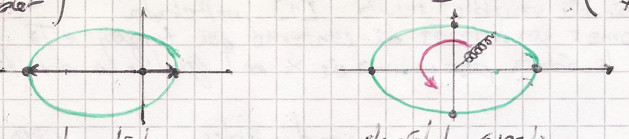
\includegraphics[scale=0.3]{images/fig_mc_orbitas_simetria_6.jpg}

El problema de Kepler da órbita cerrada elíptica siempre si $ E < 0 $ con origen en un foco (centro de fuerzas en un foco).
Tiene dos puntos apsidales y da una oscilación completa para cerrar una vuelta.

El oscilador armónico 3D da órbita cerrada con elipse con origen en el centro (centro de fuerzas en el centro). Tiene 
cuatro puntos apsidales y necesita dos oscilaciones para cerrar una vuelta.


% =================================================================================================
\section{Solución a partir de las ecuaciones de Euler-Lagrange}
% =================================================================================================

\[
	m \ddot{r} -\frac{L^2}{m r^3} -\dpar{V}{r}= 0 
\]
\[
	d \phi = \frac{L}{m r^2} dt \qquad \longrightarrow \quad  \dpar{\phi}{r}\dpar{r}{t}  = \frac{L}{m r^2}
\]
\[
	\frac{d}{t}(\dot{r}) = \frac{L}{m r^2} \frac{d}{\phi}(\dot{r})
\]
\[
	m \dtot[2]{r}{t} -\frac{L^2}{m r^3} = -\dpar{V}{r}
\]
\[
	\frac{L}{r^2} \frac{d}{\phi}\left( \dtot{r}{t} \right) -\frac{L^2}{m r^3} = -\dtot{V}{r}
\]
\[
	\frac{L}{r^2} \frac{d}{\phi}\left( \frac{L}{m r^2}\dtot{r}{\phi} \right) -\frac{L^2}{m r^3} = -\dtot{V}{r}
\]
y acá probamos el conveniente cambio de variables
\[
	U = \frac{1}{r} \qquad dU = -\frac{1}{r^2} dr 
	\qquad \dtot{U}{\phi} = -\frac{1}{r^2}\dtot{r}{\phi} = -U^2\dtot{r}{\phi}
\]
\[
	U^2 L \frac{d}{d\phi} \left\{ -\frac{L}{m}\dtot{U}{\phi} \right\} - \frac{L^2}{m r^3} U^3 = F(1/U)
\]
\[
	- \frac{U^2 L^2}{m} \dtot[2]{U}{\phi} - \frac{L^2}{m r^3} U^3 = F(1/U)
\]
\[
	- \frac{U^2 L^2}{m} \left[ \dtot[2]{U}{\phi} + U \right] = F(1/U)
\]
o bien
\[
	\left[ \dtot[2]{U}{\phi} + U \right] = - \frac{F(1/U) m}{U^2 L^2}. 
\]

En el caso del potencial de Kepler será 
\[
	\left[ \dtot[2]{U}{\phi} + U \right] = - \frac{K m}{L^2},
\]
es decir que el miembro derecho es una constante. Sale fácil entonces.

\subsection{elipses y velocidad areolar}
\notamargen{Reubicar este material}

\[
	r = \frac{a(1-e^2)}{1 + e\cos\vp}
\]
y la excentricidad es 
\[
	\begin{cases}
	e = 0 \qquad \text{ círculo } \\
	0 < e < 1 \qquad \text{ elipse } \\
	e = 1 \qquad \text{ parábola } \\
	e > 0 \qquad \text{ hipérbola }
	\end{cases}
\]

En términos de la energía y para un potencial $ V = - Cr^{-1}$ la excentricidad se puede reescribir como 
\[
	e = \sqrt{ 1 + \frac{2EL^2}{\mu C^2} }
\]

El lagrangiano para el radio equivalente [?] era
\[
	\Lag = \frac{1}{2} M \vb{R}_{\text{cm}} + \frac{1}{2} \mu (\dot{r}^2 + r^2 \dot{\vp}^2) + \frac{C}{r}
\]
pero si me sitúo en el centro de masas se reduce a 
\[
	\Lag = \frac{1}{2} \mu (\dot{r}^2 + r^2 \dot{\vp}^2) + \frac{C}{r}
\]
y la ecuación de movimiento para $ \vp $ al ser variable cíclica resulta una conservación,
\[
	\dpar{\Lag}{\dot{\vp}} = \ell = \mu r^2 \dot{\vp}
\]

% =================================================================================================
\section{Velocidad areolar}\index{Velocidad areolar--}
% =================================================================================================

\[
	\dot{\phi} = \frac{L}{m r^2}
\]
\begin{figure}[hbt]
	\begin{center}
	\includegraphics[width=0.4\textwidth]{images/fig_mc_velareolar.pdf}	 
	\end{center}
	\caption{}
\end{figure} 
Aproximo por un triángulo.
De la figura puede verse que 
\[
	dA = \frac{1}{2} r^2 d\phi 
\]
y  entonces
\[
	\dtot{A}{t} = \frac{1}{2} r^2 \dtot{\phi}{t} = \frac{1}{2} r^2 \dot{\phi} = \frac{1}{2}\frac{\ell}{\mu} = cte.
\]

La velocidad areolar es constante. Luego, integrando en un período $\tau$ se tiene que el área $A$ de la elipse es
\[
	A = \frac{\ell \tau}{2\mu}
\]
y como geométricamente ésta es 
\[
	A = \pi a b = \frac{ \pi C \ell }{\sqrt{ 8 \mu |E|^3 }}
\]
y además 
\[
	\tau = \frac{ \pi C \sqrt{\mu } }{ \sqrt{ 8 |E|^3 } }
\]
entonces el período verifica 
\[
	\tau^2 \sim \frac 1 {|E|^{3}}.
\]

\begin{ejemplo}{\bf Problema 1 (con órbita circular)}

Si $r=cte.$ entonces $\overline{T}=T$ y $\overline{V}=V$ en cuyo caso es $E = T + V = V/2$. En el caso de frenado [?] la partícula
tiene $E=V/2$ antes de frenar y luego del frenado $E=V$ (solamente potencial).

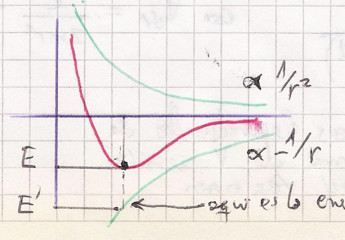
\includegraphics[scale=0.3]{images/fig_mc_potencial_energy.jpg}

Ahora supongo un problema equivalente (problema elíptico de cierto semieje). El nuevo sistema son dos masas en una
órbita elíptica que se va achatando.
\[
	\tau = \frac{ 2 \pi \mu C }{\sqrt{ 8 \mu |E|^3 }} \qquad \qquad 
	\tau' = \frac{ 2 \pi \mu C }{\sqrt{ 16 \mu |E|^3 }}
\]
y entonces
\[
	\frac{\tau}{\tau'} = \left( \frac{1}{2\sqrt{2}} \right)^{-1}
\]

Conozco esta relación 
\[
	E^{'3/2} = 2^{2/3} E
\]
\[
	\tau' = \frac{\tau}{2\sqrt{2}}.
\]

El período depende solo del semieje $a = C/(2|E|)$

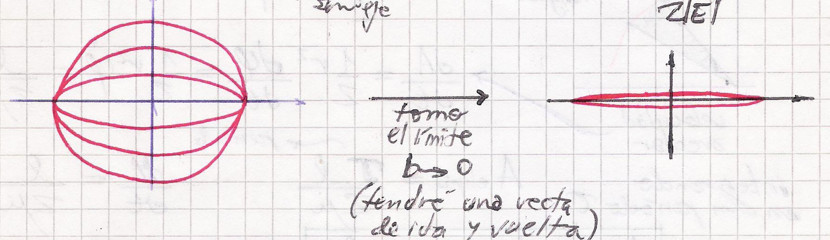
\includegraphics[scale=0.3]{images/fig_mc_potencial_energy_elipses.jpg}

Ahí tendré medio tiempo calculado porque {\it voy y vengo}
\[
	\frac{\tau'}{2} = \frac{\tau}{4\sqrt{2}} \equiv t_\text{ colisión }
\]

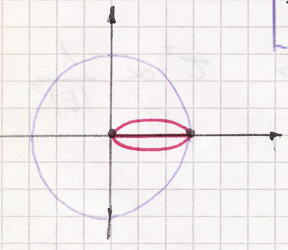
\includegraphics[scale=0.3]{images/fig_mc_potencial_energy_elipses2.jpg}

\end{ejemplo}



% =================================================================================================
\section{Las fuerzas centrales y las leyes de Kepler}
% =================================================================================================

Tenemos 
\[
	\int d\phi = \int \frac{(L/Mr^2)}{\sqrt{ \frac{2}{m}(E - V_{\text{eff}})}} dr	\qquad
	\dtot[2]{U}{\phi} + U  = - \frac{F(1/U) m}{U^2 L^2} \quad U = 1/r
\]
que es simétrica respecto a $\phi$ y $-\phi$. Esto determina una simetría orbital si
tomamos
\[
	U(\phi=0) = U_0 	\qquad		\left. \dtot{U}{\phi} \right|_{\phi=0}= 0
\]
lo cual significa que $U_0$ es un extremo (punto apsidal).

Calculemos ahora el ángulo que recorre una oscilación completa,
\[
	\Delta \phi = 2\int_{r_m}^{r_M} \frac{(L/Mr^2)}{\sqrt{ \frac{2}{m}(E - V_{\text{eff}})}} dr
\]

Si $\Delta \phi = 2 q $ siendo $q= (m/n)\pi $ son $m,n \in \mathbb{Z}$ entonces
\[
	\Delta \phi = 2 \frac{m}{n} \pi 
\]
\[
	\frac{m}{n} = \frac{2\pi}{\Delta \phi}
\]
y esto significaría que la órbita se cierra.

La ecuación a resolver es 
\[
	\dtot[2]{U}{\phi} + \left( U  - \frac{k m}{L^2} \right) = 0.
\]
Si consideramos una nueva variable 
\[
	\beta = U  - \frac{k m}{L^2}
\]
la anterior pasa a 
\[
	\dtot[2]{\beta}{\phi} + \beta = 0
\]
y es fácil ver que la solución es
\[
	\beta = A \cos( \phi -\phi_0 ),
\]
o bien 
\be
	U(\phi) = \frac{km}{L^2} +  A \cos( \phi -\phi_0 ),
	\label{sol_general}
\ee
donde $A,\phi_0$ son constantes. Ahora bien, la expresión \eqref{sol_general} es la solución general,
necesitamos proveer las condiciones iniciales para fijar $ A, \phi_0 $. Propongamos $ \phi_0 = 0 $
punto apsidal.
\notamargen{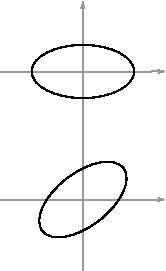
\includegraphics[width=0.3\textwidth]{images/fig_mc_detalle_elipses.pdf}
Eligiendo el punto $\phi_0 =0$ obtenemos una elipse como la de arriba.
}
Luego podemos utilizar $r_m, r_M$ lo cual determina $U_m, U_M$ respectivamente, cuyos valores son 
\[
	U^M_m = \frac{km}{L^2} \left( 1 \pm \sqrt{1 + \frac{2EL^2}{k^2 m} }\right)
\]
y esto nos permite fijar $A$. Incorporando esto en \eqref{sol_general} y recordando que $U(\phi) =1/r$ 
se tiene 
\[
	\frac{1}{r} = \frac{km}{L^2}\left( 1 +  \sqrt{1 + \frac{2EL^2}{k^2 m} } \cos( \phi ) \right),
\]
que no es otra cosa que la ecuación de una elipse en coordenadas polares con origen en un foco.
Veámoslo.

% \[
% 	\frac{1}{r} = \frac{km}{L^2} +  A \cos( \phi -\phi_0 )
% \]
% y habría que usar $r_m, r_M$ para evaluar $A$.

Las elipses verifican 
\[
	\frac{x^2}{a^2} + \frac{y^2}{b^2} = 1	\qquad \sigma^2 = a^2 - b^2
\]
donde $\sigma$ es la semi-distancia focal. Definiendo $ \sigma/a \equiv \varepsilon$ (la excentricidad) 
se puede expresar
\[
	b = a \sqrt{ 1 - \varepsilon^2 }
\]
\notamargen{Falta el sistema de coordenadas en el foco $f'$. Revisar quién es $EL$.}
\begin{figure}[hbt]
	\begin{center}
	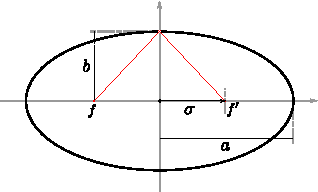
\includegraphics[width=0.4\textwidth]{images/fig_mc_elipse_1.pdf} \hspace*{2em}	 
	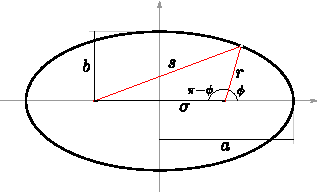
\includegraphics[width=0.4\textwidth]{images/fig_mc_elipse.pdf}	 
	\end{center}
	\caption{}
	\label{fig_mc_elipse}
\end{figure} 

Por otro lado, usando el teorema del coseno para el triángulo definido en la Figura \ref{fig_mc_elipse} es 
\[
	s^2 = (2\sigma)^2 + r^2 - 4\sigma r \cos( \pi - \phi )
\]
y como $s+r$ es la distancia que se mantiene constante e igual, entre otras, a $2a$ se sigue que 
\[
	( 2a -r )^2 = 4\sigma^2 + r^2 + 4\sigma r \cos(\phi)
\]
cuya simplificación conduce a
\[
	\frac{1}{r} = \frac{1 + \varepsilon \cos (\phi)}{a(1-\varepsilon)} = \frac{a}{\phantom{^a}b^2} \left( 1 + 
\varepsilon \cos (\phi) \right)
\]
la cual es la ecuación de una elipse.

\notamargen{Acá hay que hacer un laburo muy importante.}
% \begin{figure}[hbt]
% 	\begin{center}
% 	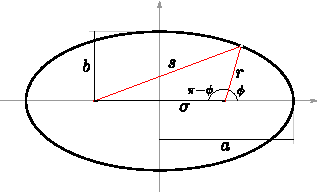
\includegraphics[width=0.4\textwidth]{images/fig_mc_elipse.pdf}	 
% 	\end{center}
% 	\caption{}
% \end{figure} 

Entonces en resumen, las leyes de Kepler son
\begin{enumerate}
 \item Los planetas giran en órbitas elípticas con el Sol en uno de sus focos. Esto es común de los potenciales del 
tipo 
	\[
		V \propto 1/r
	\]
 \item El radio vector recorre áreas iguales en tiempos iguales
	\[
		\delta A = \frac{1}{2} r^2 \delta \phi \quad \longrightarrow \quad \dtot{A}{t} = \frac{r^2}{2} 
\dot{\phi} = \frac{L}{2m} (cte.)
	\]
	Esto es una característica de todo potencial central.
 \item El cubo del semieje mayor de la órbita de un planeta es proporcional al cuadrado del período empleado en 
recorrerla.
	La ecuación anterior, que da la velocidad areolar, se puede integrar como 
	\[
		\int dA  = \frac{L}{2m} \int dt
	\]
	que conduce a 
	\[
		\pi a b = \frac{L}{2m} \tau \qquad \longrightarrow \qquad a = \frac{L\tau}{2\pi b m}, 
	\]
	y luego, como $k m /L ^2 = a/b^2$ llegamos a 
	\[
		a^3 = \frac{k}{m} \frac{1}{4\pi^2} \: \tau^2 = \frac{GM}{4\pi^2} \tau^2
	\]
 y esto es independiente de la masa del planeta.
 
Como $a$ depende de $L$ se tiene que dependiendo de la energía $E$ tendré órbitas como las ilustradas debajo
todas las cuales tienen la misma energía 
\[
	a = \frac{1}{2}(r_M + r_m) = -\frac{k}{2E}
\] 

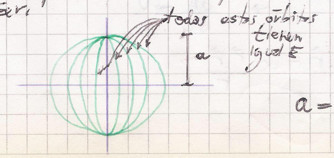
\includegraphics[scale=0.3]{images/fig_mc_orbitas_elipticas.jpg}

\notamargen{Esto estaba en la carpeta pero no lo entiendo bien del todo. Tal vez ilustración de la elipse con 
el sistema coordenado en el origen.}
 Para una elipse con el sistema coordenado en el centro se tiene 
 \[
	\frac{1}{r^2} = \frac{1}{b^2}( 1-\varepsilon^2 \cos^2 (\phi) )
 \]
 
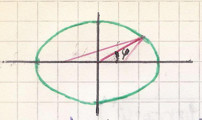
\includegraphics[scale=0.3]{images/fig_mc_orbitas_elipticas_2.jpg} 
 
 Trabajamos más con la elipse,
 \[
	r_M + r_m = 2a
 \]
 \[
	E = \frac{L^2}{2mr^2} - \frac{k}{r}	\qquad\qquad E - \frac{L^2}{2m} U^2 - kU = 0
 \]
 \[
	\frac{1}{r_{m,M}} = \frac{ \frac{2mkE}{L^2} \mp \sqrt{ \left(\frac{2mkE}{L^2}\right)^2 + \frac{8mE}{L^2} } }{2}
 \]
 \[
	\frac{1}{r_{m,M}} = \frac{mEk}{L^2} \left( 1 \pm \sqrt{1 - \frac{2L^2}{mEk^2}}\right) 
 \]
 y acá constatamos que representa una elipse; es decir que las órbitas son elípticas.
\end{enumerate}

\begin{ejemplo}{\bf Problema 1 de central forces}

Conviene pasarlo a un problema equivalente para una partícula {\it masa reducida} en términos del centro de masa.
\[
	E = \frac M 2 V_{cm}^2 + \frac \mu 2 ( \dot{r}^2 + r^2\dot{\theta}^2 ) + V( r )
\]
\[
	\tau = \frac{2\pi R}{R\dot{\theta}}
\]

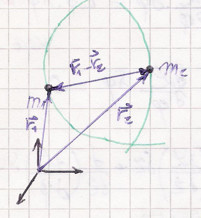
\includegraphics[scale=0.4]{images/fig_mc_central_forces1.jpg}

\[
	E = \frac 1 2 \mu(\dot{r}^2 + r^2\dot{\theta}^2 ) + \frac K r
\]
Al detenerlas,
\[
	E = - \frac K r
\]
y al rearrancar
\[
	E = \frac 1 2 \mu \dot{r}^2 - \frac K r
\]
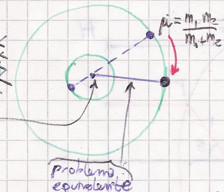
\includegraphics[scale=0.4]{images/fig_mc_central_forces2.jpg}

Para la integración le pongo el signo negativo puesto que corresponde a la situación física correcta
\[
	\dtot{r}{\tau} = -\sqrt{ \frac 2 \mu \left(E + \frac K r \right) }
\]
Integración a ambos miembros lleva a
\[
	\int_0^\tau dt = - \int_R^0 \frac{dr}{ \sqrt{ \frac 2 \mu \left(E + \frac K r \right) } }
\]
o bien a 
\[
	\tau' = \sqrt{\frac{\mu}{2}} \sqrt{\frac{R}{K}} \int_R^0 \sqrt{\frac{r}{R-r}} dr
\]

Con el cambio de variables $U=\sqrt{R-r}$ que lleva al diferencial 
\[
	dU = \frac{-dr}{2\sqrt{R-r}}
\]
la integral resulta en 
\[
  	2 \left( \frac{ \mu R }{ 2K } \right) \int_0^{\sqrt{R}} \sqrt{ R - U^2 } dU =
 	2 \left( \frac{\mu R}{2K}\right) \left( \frac{ U\sqrt{R-U^2} }{2} + \frac{R}{2} 
 	\asen\left( \frac{U}{\sqrt{R}}\right) \right)
\]
que se ha buscado en tablas.
Luego,
\[
	\tau' = \sqrt{ \frac{\mu R}{2K} }\frac{R\pi}{2}
\]
y las ecuaciones de Newton,
\[
	\frac{K}{R^2} = \mu R\dot{\theta}^2 
\]
de la cual se puede despejar $\dot{\theta}$ para obtener
\[
	\tau = 2 \pi R \sqrt{\frac{\mu R}{K}}
\]
de manera que 
\[
	\frac{ \tau }{ \tau' } = 4 \sqrt{ 2 }.
\]
\end{ejemplo}

\begin{ejemplo}{\bf Problema 4 de central forces}

Consideramos un potencial de la forma 
\[
	V(r) = \frac{K}{r^2}
\]
que es un potencial repulsivo puesto que 
\[
	F(r) = -\dpar{V}{r} = \frac{2K}{r^3}
\]
implica que {\it aleja a la partícula}.
Como es central, conserva $ L = m r^2 \dot{\theta} $ se puede escribir la energía como
\[
	E = \frac 1 2 m ( \dot{r}^2 + r^2 \dot{\theta}^2 ) + \frac K {r^2} = \frac{ m \dot{r}^2 }{2} +
	\left( \frac{ \ell }{ 2 m r^2 } + \frac{ K }{ r^2 } \right)
\]

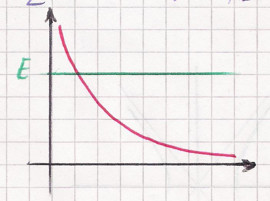
\includegraphics[scale=0.3]{images/fig_mc_potencial_central_4.jpg}

Luego,
\[
	\dot{r} = \sqrt{ \frac{2E}{m} - \frac{2L}{2m^2r^2} - \frac{2K}{mr^2} }
\]
y entonces
\[
	m r^2 \sqrt{ \frac{2E}{m} - \frac{2L}{2m^2r^2} - \frac{2K}{mr^2} } \dtot{\theta}{r} = L
\]
de manera que 
\[
	\int_0^{\theta} d\theta = \frac{L}{\sqrt{2m}} \int_{r_0}^{r} \frac{dr}{r^2( E - L/(2mr^2) - K/r^2 )^{1/2}}
\]

Con el cambio de variables $ U = 1 / r $
\[
	\theta = -\frac{L}{\sqrt{2m}} \int_{1/r_0}^{1/r} \frac{ dU }{ [ E - U^2( L/(2m) + K )]^{1/2} }
\]

Integrada da
\[
	\theta = \frac{L}{m\sqrt{2Km + \frac{L^2}{m^2}}}
	\left( \acos\left[ \frac{ \sqrt{2Km + L^2/(m^2)} }{r_0\sqrt{2E/m}} \right] - 
	\acos\left[ \frac{\sqrt{2Km + L^2/(m^2)}}{r\sqrt{2E/m}}\right] \right).
\]

Tomo $r_0$ punto de retorno
\[
	E = \left( \frac{L^2}{2mr_0^2} + \frac{K}{r_0^2} \right)
\]
y entonces
\[
	r_0 = \sqrt{ \frac L {2mE} + \frac K E }
\]
\[
	\theta = \frac{L}{m\sqrt{2Km + \frac{L^2}{m^2}}} \acos\left(\frac{r_0}{r}\right)
\]
y se puede despejar
\[
	r = \frac{ r_0 }{\cos( \theta m / L \sqrt{ 2 m K + L^2 / m^2 } )}
\]
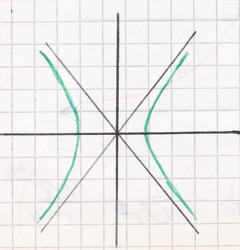
\includegraphics[scale=0.3]{images/fig_mc_potencial_central_4_orbitas.jpg}

Continuamos con el problema [esto sacarlo, je!]

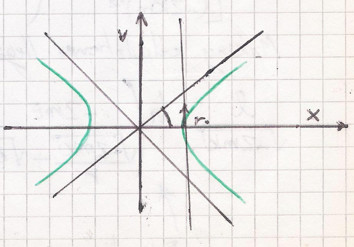
\includegraphics[scale=0.3]{images/fig_mc_potencial_central_5_orbitas.jpg}
\[
	r = \frac{ r_0 }{ \cos( \vp \sqrt{ 2 m^3 K / L^2 + 1 } ) }
\]
\notamargen{Ojo, chequear esta expresión porque en la carpeta está distinta!}

Vemos el comportamiento asintótico, si $ K = 0 $ entonces
\[
	r = \frac{ r_0 }{ \cos \vp }.
\]
Si el potencial es atractivo, por ejemplo $ V(r) = -\frac{K}{r^2}$ entonces se puede escribir 
\[
	E = \frac{1}{2} m \dot{r}^2 + \frac{K'}{r^2},
\]
donde 
\[
	K' = \left( \frac{L^2}{2m} - \frac{K}{} \right).
\]
Entonces la velocidad será 
\[
	\dot{r} = \sqrt{ \frac{2}{m}\left( E - \frac{K'}{r^2} \right) }
\]

A partir de la ecuación para el momento angular, $ m r^2 \dot{\vp} = L $ podemos llegar a la integral para $\vp(r)$ [esto creo que ya se hizo en la 
teoría, en dicho caso citar, sino hacer en detalle]
\[
	\int d\vp = \int \frac{L}{m} \frac{ dr }{ r^2 \sqrt{ \frac{2}{m}\left( E - \frac{K'}{r^2} \right) }}
\]
Con el reemplazo usual $r = 1/U$ se llega a 
\[
	\vp = -L \int \frac{ dU }{ ( 2mE - K'mU^2 )^{1/2}}.
\]

Si $L^2 > 2mK$ es 
\[
	\frac{L^2 - 2mK}{2m} > 0 \qquad K'>0
\]
y tengo un caso similar al anterior (en la página precedente[sic carpeta?]). En cambio si $ L^2 < 2mK $ se tiene $ K' < 0 $.
Usano la ayuda para la integral [refiere al enunciado en la guia?] que se hace entre $r_0$ y algún $r$ final resulta 
\[
	\vp =  \frac{L}{\sqrt{-2mK'}} \log \left( \frac{-2mE}{ \sqrt{ -2mK'/r } + \sqrt{2mE - K'/r^3} }\right)
\]
y esto dice que la partícula cae al origen describiendo una espiral. En el origen es $\dot{\vp} \to \infty$

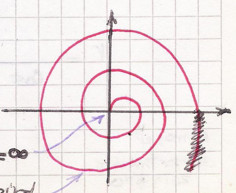
\includegraphics[scale=0.3]{images/fig_mc_potencial_central_6_orbitas.jpg}

Dicho esto, se puede calcular el tiempo que tarda en caer al origen a partir de la ecuación para $\dot{r}$
\[
	-\int_{r_0}^0 \frac{1}{\sqrt{ 2/m ( E - K'/r^2 ) }} = \int_0^{t_f} dt
\]
Como la energía se conserva puede utilizarse su valor inicial, $E=K'/r_0^2$ de modo que el LHS de la ecuación anterior es
\[
	t_f = -\sqrt{ \frac{m}{-2K'} } \int_{r_0}^0 \frac{ r_0 r }{\sqrt{ r_0^2 - r^2 }} = r_0^2 \sqrt{\frac{m}{-2K'}}.
\]
\end{ejemplo}

% =================================================================================================
\section{Teorema del virial}
% =================================================================================================

Se aplica a sistemas de muchas partículas. Defino 
\[
	G \equiv \vb{p}_i \cdot \vb{x}_i
\]
de modo que como $ \dot{\vb{p}}_i = \vb{F}_i $ se tiene 
\[
	\dtot{G}{t} = \dtot{\vb{p}_i}{t} \cdot \vb{x}_i + \vb{p}_i \dtot{\vb{x}_i}{t}
\]
y se puede ver que el último miembro del RHS es $ \vb{p}_i \dot{\vb{x}}_i = m_i v_i^2 = 2T$ donde $T$ es la energía cinética del sistema.
Luego 
\[
	\dtot{G}{t} = \sum_i^N \dtot{\vb{p}_i}{t} \cdot \vb{x}_i + 2 T
\]

Defino el valor medio temporal de una cantidad $A$ según 
\[
	\bar{A} = \lim_{\tau \to \infty} \frac{1}{\tau} \int_0^\tau A(t) dt
\]
[Pasar esto a Apéndice!!].
\[
	\overline{G} = \frac{1}{\tau} \int_0^\tau \dtot{G}{\tau} dt = \overline{ 2 T } + \overline{ \sum_i^N \vb{F}_i \cdot \vb{x}_i }
\]
Pero el integrando en el LHS es un diferencial total, entonces 
\[
	\frac{1}{\tau} \left( G(\tau) - G(0) \right) = \overline{ 2 T } + \overline{ \sum_i^N \vb{F}_i \cdot \vb{x}_i }
\]

Si ahora estoy trabajando con un sistema que realiza un movimiento períódico, entonces en $\tau$ definido como ese período tiene 
\[
	\overline{ 2 T } + \overline{ \sum_i^N \vb{F}_i \cdot \vb{x}_i } = 0
\]
lo cual lleva a el teorema del virial\index{Virial, teorema del}
\[
	\overline{ T }  = - \frac{1}{2} \overline{ \sum_i^N \vb{F}_i \cdot \vb{x}_i }.
\]

También es cero si el mov. [?]

La temperatura media es 
\[
	\overline{T} = \frac 3 2 N k T'
\]
para partículas en un recipiente. La fuerza es por los golpeteos (la temperatura en realidad es microscópicamente una manifestación de golpeteo 
molecular). Si $ d\vb{F}_i = - p \hat{n}dA $ de modo que 
\[
	\frac{1}{2} \sum_i \vb{F}_i \cdot \vb{x}_i = -\frac{p}{2}\int_S \hat{n}\cdot\vb{x}dA =
	-\frac{p}{2} \int_V \nabla\cdot \vb{x} dV = - \frac{3}{2} p V
\]
y entonces, igualando con la expresión anterior de la $\overline{T}$ se tiene 
\[
	N k T = p V,
\]
que es la ecuación de estado del gas ideal.

Si ahora supongo $\vb{F} = -\nabla V$ homogénea de grado $k$
\[
	\overline{T} = -\frac{1}{2} \overline{ \sum_i^N \vb{F}_i \cdot \vb{x}_i } = 
	-\frac{1}{2} \overline{ \sum_i^N \dpar{V(\vb{x})}{\vb{x}_i} \cdot \vb{x}_i } = 
	\frac{1}{2} \overline{ k V(\vb{x} ) } = \frac{1}{2} k \overline{V}
\]
\notamargen{Acá hay que aclarar que hace la homogeneidad para transformar el gradiente en $kV$.}

Con un potencial central vale 
\[
	V = -\frac{C}{r} = -Cr^{-1},
\]
o sea que es un potencial homogéneo de grado $k=-1$. Entonces, para un movimiento periódico bajo una fuerza central,
será 
\[
	\overline{T} = -\frac{1}{2}\overline{V}
\]
de manera que $\overline{E} = \overline{T} + \overline{V} = 1/2 \overline{V}$. Para un oscilador armónico, como $k=-2$
se tiene $\overline{E} = 2\overline{T} = 2\overline{V} $



% =================================================================================================
\section{Vector de Runge-Lenz}
% =================================================================================================

Para el problema de Kepler también se conserva una cantidad llamada {\it vector de Runge-Lenz} definido como
\[
	\vb{R} = \vb{v} \times \vb{l} - \alpha \frac{\vb{x}}{x}.
\]

Luego, si le tomamos la derivada temporal, resulta
\[
	\dtot{\vb{R}}{t} = \left( \dtot{\vb{v}}{t} \times \vb{l} \right) + \left( \vb{v} \times \dtot{\vb{l}}{t} \right)
	- \alpha\frac{ \vb{v} }{x} + \frac{ \alpha }{x^2} \dtot{x}{t} \vb{x}
\]
donde el último se puede poner en términos de la velocidad si utilizamos la regla de la cadena así
\[
	\dtot{|\vb{x}|}{t} = \dtot{|\vb{x}|}{x_i} \dtot{x_i}{t} = \nabla( |\vb{x}| )\cdot \vb{v} \qquad  \qquad i=1,2,3
\]

Luego, cada componente $i$-ésimo del gradiente de la norma del vector de posición tiene (en coordenadas cartesianas) la 
misma
forma; tomando como ejemplo el $i=1$
\[
	\dtot{|\vb{x}|}{x_1} = \dtot{\sqrt{x_1^2 + x_2^2 + x_3^2}}{x_1} = \frac{x_1}{|\vb{x}|},
\]
de manera que 
\[
	\nabla( |\vb{x}| ) = \frac{\vb{x}}{x} = \hat{x},
\]
el gradiente de la norma del vector es su dirección. Entonces, volviendo a la ecuación original resulta 
\[
	\dtot{\vb{R}}{t} = \left( \dtot{\vb{v}}{t} \times \vb{l} \right) + \left( \vb{v} \times \dtot{\vb{l}}{t} \right)
	- \alpha\frac{ \vb{v} }{x} + \alpha \:\vb{x} \left( \frac{ \pe{x}{v} }{x^3}\right) 
\]

Dado que $\vb{l} = \vb{x} \times m \vb{v}$ el segundo término en la anterior expresión desaparece y nos queda
\[
	\dtot{\vb{R}}{t} = \left( \dtot{\vb{v}}{t} \times [ \vb{x} \times m\vb{v} ] \right) 
	- \alpha\frac{ \vb{v} }{x} + \alpha \:\vb{x} \left( \frac{ \pe{x}{v} }{x^3}\right) 
\]

\notamargen{Aparentemente esto tiene que dar nulo pero no lo estaría viendo.}

\[
	\dtot{\vb{V}}{t} \times ( \vb{x} \times m\vb{v} ) +
	\vb{V} \times \left( \dtot{\vb{r}}{t} \times m\vb{v} + \vb{r} \times m\dtot{\vb{v}}{t} \right)
\]
pero como $\dtot{\vb{r}}{t} \times m\vb{v} = 0$ resulta lo que resulta.
\begin{figure}[hbt]
	\begin{center}
	\includegraphics[width=0.4\textwidth]{images/fig_mc_rungelenz.pdf}	 
	\end{center}
	\caption{}
\end{figure} 

El vector de Runge-Lenz siempre apunta en la misma dirección dada su constancia (ver figura).
\notamargen{Mejorar la figura!}

Escribo $ T = E - V $
\[
	r_{max} m v^2 = 2Er_{max} + 2\alpha
\]
pero 
\[
	r_{max} = \frac{2 E l^2 \alpha}{\alpha^2 m (1-\varepsilon)} = \frac{-1}{\alpha}\frac{b^2 
\alpha}{\alpha^2(1-\varepsilon)}
\]
\[
	r_{max} = - (1+\varepsilon) \alpha
\]

\[
	b^2 = a^2( 1 - \varepsilon^2 )
\]

\begin{ejemplo}{\bfseries Vector de Runge-Lenz en órbitas elípticas}
\notamargen{Este título es provisorio. Está en la carpeta en 42R.}

Sabemos que el vector de Runge-Lenz tiene la forma 
\[
	\vb{A} = \pv{V}{L} - \alpha \frac{\vb{x}}{x}
\]
y cumple 
\[
	\dtot{A}{t} = 0
\]

Veamos qué expresión tiene el módulo $ A \equiv |\vb{A}| $. Tomando el producto escalar 
\[
	\pe{A}{x} = A r \cos \theta = ( \pv{V}{L} )\cdot \vb{x} - \alpha \frac{\pe{x}{x}}{x}
\]
y reescribiendo (ciclicidad del producto vectorial)
\[
	( \pv{V}{L} )\cdot \vb{x} = \vb{L} \cdot ( \pv{r}{v} ) = \vb{L} \cdot \frac{ \vb{L} }{m} = \frac{L^2}{m}
\]
y entonces
\[
	\alpha r \left( 1 + \frac{A}{\alpha} \cos \theta \right) = \frac{L^2}{m}
\]
pero como $ (1 + \varepsilon \cos \theta ) = p / r $ es la excentricidad se tiene $ A = \varepsilon \alpha $.

\end{ejemplo}

\begin{ejemplo}{\bf Problema . Nuevo potencial}

Para el potencial 
\[
	U(r) = -\frac{\alpha}{r} + \delta U(r), \qquad |\delta U| \ll \frac{\alpha}{r}
\]
la integral resultante es
\[
	\vp = \int \frac{L dr }{r^2\sqrt{2m(E-U)-\frac{L^2}{r^2}}}
\]
pero si derivamos con respecto a un parámetro (por ejemplo $L$) se pueda cambiar la misma a 
\[
	\vp = - \dtot{}{L} \int \frac{ \sqrt{2m(E-U)- L^2} }{r^2}dr
\]
y esta segunda se comporta mejor que la primera.

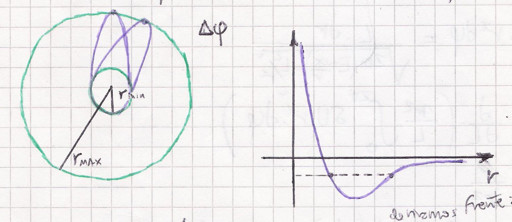
\includegraphics[scale=0.35]{images/fig_mc_potencial_central_problema.jpg}

Una órbita no cerrada, a la larga, pasas por todos los putnos dentro del área barrida.

Ahora se trabajará el integrando anterior
\[
\sqrt{ 2m \left(E+ \frac{\alpha}{r}\right) - 2m\delta U - \frac{L^2}{r^2} } =
\sqrt{ 2m \left(E+ \frac{\alpha}{r}\right) - \frac{L^2}{r^2} } 
\sqrt{ 1 - \frac{ 2m\delta U }{ 2m \left(E+ \frac{\alpha}{r}\right) - \frac{L^2}{r^2} }  }
\]

Se puede considerar una expansión de Taylor en la segunda raíz de manera que 
\[
	\vp = - \dtot{}{L}\left[ \int 
	\sqrt{ 2m \left(E+ \frac{\alpha}{r}\right) - \frac{L^2}{r^2} } dr -
	m \int \frac{ \delta U dr }{ \sqrt{ 2m \left(E+ \frac{\alpha}{r}\right) - \frac{L^2}{r^2} }  }
	\right]
\]
\[
	\vp = 2 \pi + m \dtot{}{L} 
	\int \int \frac{ \delta U dr }{ \sqrt{ 2m \left(E+ \frac{\alpha}{r}\right) - \frac{L^2}{r^2} }  }
\]
donde el primer resultado, $2\pi$, proviene de la solución del problema de Kepler y el segundo es 
un término $\Delta \vp$ que dependrá de la forma de la perturbación.
Considerando perturaciones del tipo
\[
	\delta U = \frac{\beta}{r^2} \qquad \qquad \delta U = \frac{\gamma}{r^3}
\]

Antes de proceder es conveniente hacer un pasaje de la integral. Recordando que se tenía
\[
	dt = \frac{dr}{ \sqrt{ 2m \left(E+ \frac{\alpha}{r}\right) - \frac{L^2}{r^2} } }
\]
y que la conservación del momento angular $L$ implicaba
\[
	L = mr^2\dot{\theta}{t},
\]
si pasamos $\theta$ a $\vp$ entonces $dt = ( mr^2/L ) d\vp $ y consecuentemente
\[
	m r^2 d\vp = \frac{ L dr }{ \sqrt{ 2m \left(E+ \frac{\alpha}{r}\right) - \frac{L^2}{r^2} } }
\]
de forma que 
\[
	\Delta \vp = \dtot{}{L} \left( \frac{m^2}{L} \int_0^{2\pi} \delta U r^2 d\vp \right).
\]

Regresando ahora a las formas específicas planteadas, vemos que en el primer caso es
\[
	\Delta \vp = \beta m^2 2 \pi \dtot{}{L}\frac{1}{L} = - \frac{2\pi m^2 \beta}{L^2},
\]
mientras que para el segundo la integral resulta en
\[
	\gamma \int_0^{2\pi} \frac{d\vp}{r(\vp)}, 
\]
que se puede hacer explícitamente recordando que $p = L^2/(m\alpha)$ y
\[
	\frac p r = 1 + \varepsilon \cos \vp
\]
y entonces 
\[
	\frac 1 r = \frac{m\alpha}{L^2} + \frac{\varepsilon \cos \vp}{L^2},
\]
todo lo cual lleva a que 
\[
	\Delta \vp = \dtot{}{L}\left( \frac{m^3}{L^3} \gamma \alpha \right) =
	-\frac{3m^2\gamma \alpha}{L^4}.
\]
\end{ejemplo}

% =================================================================================================
\section{Precesión [acomodar]}
% =================================================================================================

Este movimiento, ver figura, corresponde a una oscilación completa de $r_m$ a $r_M$ y vuelta.
La precesión de un punto de la órbita se aplica a órbitas en las cuales puede pensarse que la órbita se mueve 
como un todo en su figura. La magnitud $\delta \vp / \tau_r$ es la velocidad angular de precesión.

\[
	\mbox{ Ilustración 45R inferior }
\]

% =================================================================================================
\section{Orbitas de potenciales centrales}
% =================================================================================================

\[
	V(r) = -\frac{\alpha}{r}
\]
\[
	V(r) = \frac{ k r^2 }{2}
\]
Estos dos casos dan órbitas cerradas. Pero hay otros potenciales interesantes.
El potencial de Yukawa
\[
	V(r) = - \frac{\euler^{-\lambda r}}{r^\alpha}
\]
que es aproximadamente como un potencial coulombiano apantallado ($\alpha=1,\lambda=0$).
Otro es el oscilador no armónico\index{Oscilador no armónico}
\[
	V(r) = r^\alpha
\]
Algunos casos se muestran bajo estas líneas

\begin{figure}[hbt]
	\begin{center}
	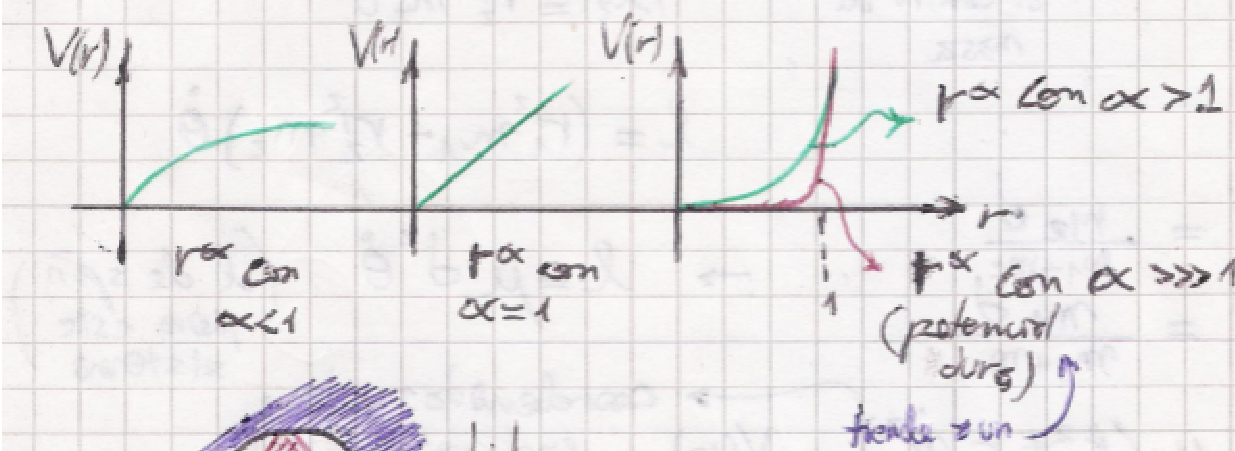
\includegraphics[width=0.6\textwidth]{images/fig_mc_potenciales_otro.pdf}
	\end{center}
	\caption{Algunas curvas de potenciales anarmónicos $ r^\alpha $.}
\end{figure}

Da órbita que no se cierra en un billar elíptico.

\begin{figure}[hbt]
	\begin{center}
	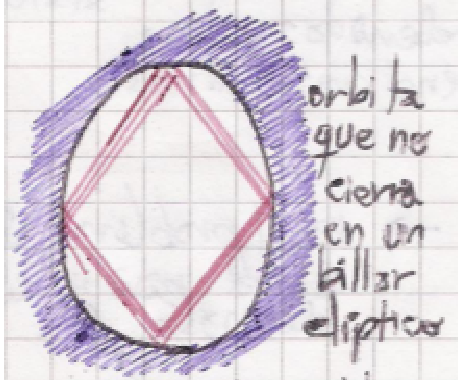
\includegraphics[width=0.4\textwidth]{images/fig_mc_billar.pdf}
	\end{center}
	\caption{.}
\end{figure}

% =================================================================================================
\section{Reducción del problema de dos cuerpos a uno equivalente}
% =================================================================================================

Para dos partículas de masas $ m_1 $ y $ m_2 $ sometidas a una fuerza central 
\[
	\vb{F}_{21} = F(r) \hat{r}_{21} \qquad \qquad F(r) = -\dtot{V(r)}{r}
\]
siendo $x \equiv |\vb{x}_2-\vb{x}_1|$ la distancia relativa.

\begin{figure}[hbt]
	\begin{center}
	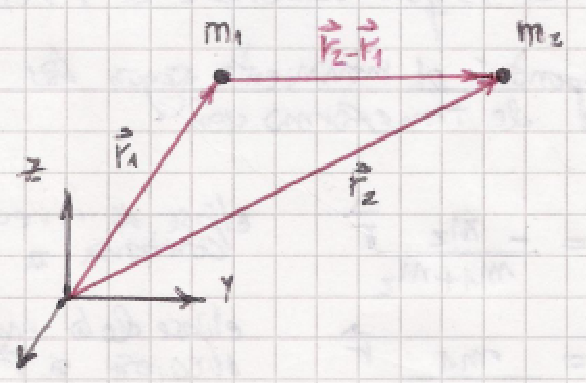
\includegraphics[width=0.4\textwidth]{images/fig_mc_prob_equiv_scheme.pdf}	 
	\end{center}
	\caption{.}
	\label{fig_mc_prob_equiv_scheme}
\end{figure} 

La energía del sistema será de la forma  $ E = T_1 + T_2 + V(r) $ pero se puede expresar según 
$ E = T_{cm} + T_{rel} + V(r) $; es decir separando la energía cinética en el aporte del centro de
masa más un aporte que depende de la distancia relativa entre los cuerpos.
De modo idéntido para el momento angular podemos pasar de $ L_{total} = L_{cm} + L_{spin} $ donde el
momento angular de spin es el referido al movimiento en torno al centro de masas.

\notamargen{Revisar y consolidar toda la notación aquí, que está mezclada.}
Consideramos el siguiente sistema de coordenadas,
\[
	r \equiv | \vb{r}_2 - \vb{r}_1 | \qquad	\qquad  \dot{r} \equiv | \dot{\vb{r}}_2 - \dot{\vb{r}}_1 |
\]
donde el sistema centro de masas es
\[
	\vb{R}_{cm} = \frac{ m_1\vb{r}_1 + m_2\vb{r}_2 }{ m_1 + m_2 }	\qquad 
	M \vb{V}_{cm} =  m_1\vb{v}_1 + m_2\vb{v}_2 
\]
\[
	0 = m_1\vb{r}_1' + m_2\vb{r}_2'
\]
que provocan
\[
	\vb{r}_1' = -\frac{m_2}{m_1}\vb{r}_2' \qquad   \vb{r}_2' = -\frac{m_1}{m_2}\vb{r}_1' 
\]
dando unas $r$ relativas
\be
	\vb{r} = \vb{r}_1' - \vb{r}_2' = -\frac{ m_1 + m_2 }{ m_1 } \vb{r}_2' = -\frac{ m_1 + m_2 }{ m_2 } \vb{r}_1'.
	\label{r_relativas}
\ee

\begin{figure}[hbt]
	\begin{center}
	\includegraphics[width=0.4\textwidth]{images/fig_reduccion.pdf}	 
	\end{center}
	\caption{Sistema coordenado para la reducción del problema de dos cuperpos al de uno equivalente.}
\end{figure} 

Luego, como la energía se conserva (el $V_{cm}=cte.$) podemos escribir
\[
	E = \frac{1}{2} m_1 \dot{\vb{r}}_1^2 + \frac{1}{2} m_2 \dot{\vb{r}}_2^2 + V(r)
\]
\[
	E = \frac{1}{2} m_1 ( \dot{\vb{R}} + \dot{\vb{r}}_1' )^2 + \frac{1}{2} m_2 ( \dot{\vb{R}} + \dot{\vb{r}}_2' )^2 
+ V(r)
\]
\[
	E = \frac{1}{2} m_1 ( {\vb{V}} )^2 +  \frac{1}{2} m_1 ( \dot{\vb{r}}_1' )^2 + 
		\frac{1}{2} m_2 ( {\vb{V}})^2 + \frac{1}{2} m_2 (\dot{\vb{r}}_2' )^2 + V(r)
\]
\[
	E = \frac{1}{2} M {\vb{V}}^2 + \frac{1}{2} \frac{m_2^2}{m_1} \dot{\vb{r}}_2'^2 + \frac{1}{2} m_2 
\dot{\vb{r}}_2'^2 + V(r)
\]
\[
	E = \frac{1}{2} M {\vb{V}}^2 + \frac{1}{2} \frac{m_2 m_1}{M} \dot{\vb{r}}^2 + V(r).
\]

Pero como $E$ y la $\vb{V}$ se conservan, se tiene 
\[
	e \equiv E - \frac{1}{2} M {\vb{V}}^2 =  \frac{1}{2} \mu \dot{\vb{x}}^2 + V(r)
\]
donde $e$ es una cantidad conservada que podemos llamar la energía reducida[?].

Este último $\vb{x}$ es un vector distancia relativa. Es un problema equivalente para la partícula
centro de masas.

\begin{figure}[hbt]
	\begin{center}
	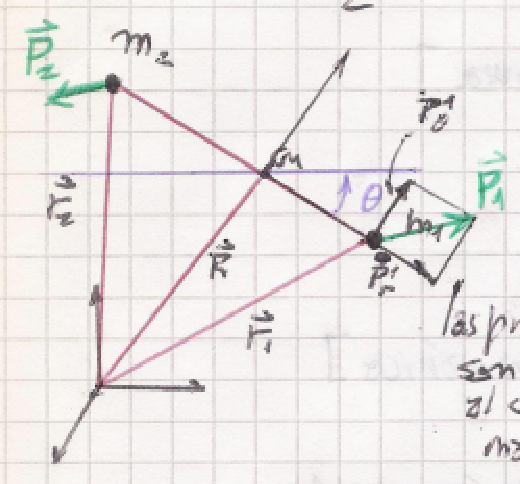
\includegraphics[width=0.4\textwidth]{images/fig_mc_prob_equiv.pdf}	 
	\end{center}
	\caption{.}
	\label{fig_mc_prob_equiv}
\end{figure} 

Podemos considerar ahora los momentos angulares de las partículas respecto de este sistema centro
de masas. Así
\[
	\vb{l}_1' = \vb{x}_1' \times \vb{p}_1 \qquad \qquad  \vb{l}_2' = \vb{x}_2' \times \vb{p}_2'
\]
y sus módulos verifican 
\[
	|\vb{l}_1'| = {x}^{2'}_1 m_1 \dot{\theta} \qquad \qquad  |\vb{l}_2'| = {x}^{2'}_2 m_2 \dot{\theta}
\]
de manera que 
\be
	\ell = ( {x}^{2'}_1 m_1 + {x}^{2'}_2 m_2 ) \dot{\theta} = \mu r^2 \dot{\theta}
	\label{mom_ang_conserv}
\ee
es el momento angular de spín para este sistema. Nótese que a partir de \eqref{r_relativas} se puede
expresar las $x'_i$ ($i=1,2$) en términos de $r$.

Luego, en coordenadas polares en el centro de masa resulta
\[
	e = \frac{1}{2} \mu ( \dot{ r}^2 + r^2\dot{\phi}^2 ) + V(r),
\]
o bien, usando \eqref{mom_ang_conserv},
\[
	e = \frac{1}{2} \mu \dot{ r}^2 + \frac{\ell^2}{2 \mu r^2 } + V(r)
\]
que no es otra cosa que el problema de fuerza central para un cuerpo de masa $\mu$.

Diremos que la {\it distancia relativa} describe una elipse. Las trayectoria reales en el espacio físico
son dos elipses confocales. Por supuesto dejan de cumplirse las leyes de Kepler en este caso.

Si como solución proponemos
\[
	V(r) = -\frac{\alpha}{r}
\]
tendré $ r = r(\phi) $ una elipse, que es lo que describe el $ r $ relativo.
Se descompondrá el movimiento según las ecuaciones de transformación
\[
	\vb{r}_1'= -\frac{m_2}{m_1+m_2} \vb{r} \qquad \text{ Elipse de dirección contraria a $\vb{r}$}
\]
\[
	\vb{r}_2'= \frac{m_1}{m_1+m_2} \vb{r} \qquad \text{ Elipse de dirección igual a $\vb{r}$}	
\]
Tendremos dos elipses confocales como muestra la figura bajo estas líneas 

\begin{figure}[hbt]
	\begin{center}
	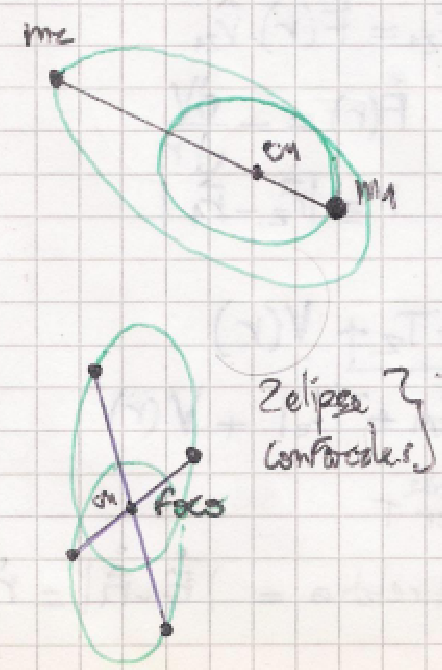
\includegraphics[width=0.4\textwidth]{images/fig_mc_elipses_confocales.pdf}	 
	\end{center}
	\caption{.}
	\label{fig_mc_elipses_confocales}
\end{figure} 

En este caso ya dejan de cumplirse las leyes de Kepler
\[
	\dtot{\mathcal{A}}{t} = \frac{\ell}{2\mu} \qquad a^3 \sim \tau^2 
\]
para la órbita relativa.
\[
	\frac{\pi a b }{\tau}= \frac{\ell}{2\mu} 
\]
\[
	b = \frac{\ell}{\sqrt{\alpha \mu}} a^{1/2} \qquad \frac{a}{b} = \frac{\mu \alpha}{\ell^2}
\]
\[
	\frac{\pi a^{3/2}}{\sqrt{\alpha \mu} \tau} = \frac{1}{2\mu}
\]
y entonces ahora se ve que no es independiente de las masas y no se puede simplificar $\sqrt{\mu\alpha}$ con
$\mu$ como ocurría en un movimiento elíptico tradicional (bajo potencial gravitatorio).
Entonces no es válida la ley de Kepler.

% =================================================================================================
\section{Dispersión}
% =================================================================================================

\subsection{preliminares--usar y destruir--}

Se supone una partícula chocando a la vez (el haz incidente no interactúa entre sí).
Se conoce las partículas incidentes por área y por tiempo $I$ y las dispersadas serán
$ D = I \int \dtot{\sigma}{\Omega} d\Omega = I \sigma$.
Se consideran coordenadas en el centro de masa.
Se trabaja en ángulos sólidos.
\notamarge{El problema 1 en página 45 parece estar hecho en la teoría, de manera que no transcribe
ahora.}

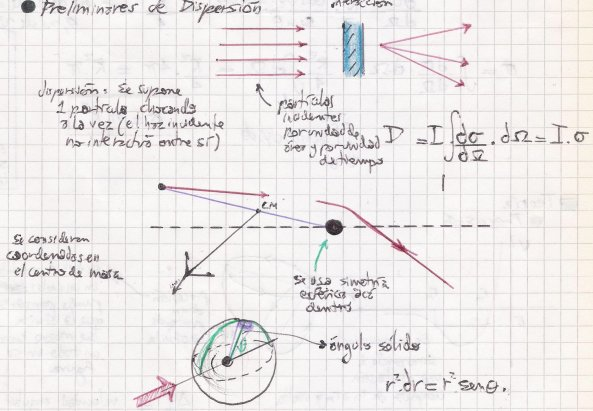
\includegraphics[scale=0.3]{images/fig_mc_dispersion_varios.jpg}

Es un tema muy importante porque permite investigar qué hay en el interior de la materia por medio
de {\it pegarle} con algo que se conoce perfectamente.
En estas situaciones el blanco es desconocido y el proyectil conocido.

Pero proyectil y blanco pueden actuar de acuerdo a un potencial. Esta interacción queda especificada
por la {\it sección eficaz de dispersión elástica}.

Veamos primeramente a lo que se llama un {\it centro dispersor} (blanco de masa tendiendo a infinito).
Al lanzar un haz de partículas (proyectiles) en primera instancia están libres y al acercarse recién se
notan los efectos.

Consideramos la dispersión de un haz de partículas de cierta energía cinética por un centro dispersor,
ver ilustración. Todas las partículas tienen la misma energía $1/2 m V_\text{ cm }$

\begin{figure}[htb]
	\begin{center}
	\includegraphics[width=0.5\textwidth]{images/fig_mc_dispersion1.pdf}	 
	\end{center}
	\caption{}
\end{figure} 


La sección eficaz diferencial es $d\sigma$ que es el número de partículas dispersadas entre 
$\chi$ y $\chi + d\chi$ por unidad de tiempo.
Pero esto depende del ancho del haz y de la cantidad de partículas del haz. Para independizarlo se
divide por la intensidad del haz (\# de partículas por área) y se construye así $d\sigma'$
\[
	d\sigma' \equiv \dtot{\sigma}{n} dA dt 
\]
y así $d\sigma'$ tiene unidades de área. Obviaremos en lo que sigue la ``''' en la notación.
Entonces, ahora, la sección eficaz diferencial, bien definida, es 
\[
	d\sigma = \frac{dN}{n}
\]
siendo $dN$ el número de partículas dispersadas entre $\chi$ y $\chi + d\chi$ por unidad de tiempo
y $n$ el número de partículas emitidas por tiempo y por área.

Si el centro dispersor tiene simetría esférica el cálculo es sencillo, puesto que se conserva el 
momento angular $L$. En realidad, ya con la simetría radial cilíndrica en torno a la dirección del 
haz basta para resolver analíticamente.
Estas suposiciones son muy fuertes y restrictivas pero a fin de cuentas este es un caso de gabinete
para formar algunas ideas.

Consideramos $d$ centro dispersor con simetría esférica (cilíndrica basta).

\[
	mbox{ \text{ Figura 46 abajo. } }
\]

Usamos como suposiciones que todo lo que emerge entre $\rho + d\rho$ - $\rho$  es dispersado entre
$\chi + d\chi$ - $\chi$, y que se conservan tanto $E$ como \vb{L}.

\begin{figure}[htb]
	\begin{center}
	\includegraphics[width=0.5\textwidth]{images/fig_mc_dispersion2.pdf}	 
	\end{center}
	\caption{}
\end{figure}

El anillo se dispersa en un sector esférico. Entonces para el anillo entre $\rho + d\rho$ - $\rho$ el
área de la corona será
\[
	A =  \pi ( (\rho + d\rho)^2 - \rho^2 ),
\]
que a primer orden (suponiendo $d\rho$ diferencial) será 
\[
	A \approx 2 \pi \rho \: d\rho.
\]

La variable $\rho$ es el llamado {\it parámetro de impacto}. Entonces
\[
	d\sigma = \frac{  2 \pi \rho \: d\rho I}{I} = 2 \pi \rho d\rho
\]
donde $I$ el número de partículas por unidad de tiempo y área
en el haz. Si obtuviese $ \rho = \rho(\chi) $ entonces inalmente
\[
	d\sigma =  2 \pi \rho(\chi) \left| \dtot{\rho}{\chi} \right| d\chi
\]
donde el módulo es porque la cantidad correspondiente será negativa. La función $\rho(\chi)$ nos dará
información sobre el potencial entre las partículas y el centro.
La función $\chi(\rho)$ se llama función deflexión.

Como se conservan la energía y el momento angular
\[
	E = \frac{1}{2} m V_\infty^2 \qquad L = m \rho V_\infty^2 
\]
aunque por supuesto al variar $\rho$ varío el momento angular $L$ de las partículas. Entonces tanto una
como otra magnitud determinan cómo se dispersan las partículas.

La conservación de $L$ implica la constancia de $\rho$ como valor asintótico para la trayectoria. El punto
apsidal es un punto tal que existe simetría de la órbita respecto al mismo.
\[
	mbox{ \text{ figura 46R izquierda} }
\]
\begin{figure}[htb]
	\begin{center}
	\includegraphics[width=0.5\textwidth]{images/fig_mc_dispersion3.pdf}	 
	\end{center}
	\caption{}
\end{figure}

Se puede calcular el ángulo $\varphi_0$ de acuerdo a 
\[
	\chi = \pi - 2\varphi_0,
\]
donde
\[
	\varphi_0 = \int_{r_m}^{\infty} \frac{L/mr^2}{\sqrt{\frac{2}{m}(E - V_{\text{eff}} )}} dr
\]
\[
	\chi = \pi - 2 \varphi_0 (\rho)
\]
e invertimos desde la última ecuación. Considerando $E = 1/2 m v_\infty$ y $ L = m \rho v_\infty $
se tiene 
\[
	V_{\text{eff}} = \frac{L}{2 m r^2} + V(r)
\]
aunque en general se desconoce $V(r)$ o el tamaño efectivo de su interacción. En esos casos se puede 
ajustar el cálculo con lo que se mide experimentalmente para tener un potencial parecido a la interacción
real.

\subsection{Esfera maciza}

Veamos el caso de una esfera maciza. Lo primero es encarar el cálculo de $\rho=\rho(\chi)$ o su inversa.
En general los cuerpos duros equivalen a un potencial del tipo
\be
	V = \begin{cases}
	     \infty \qquad \textrm{cuerpo}\\
	     \;0 \qquad \; \textrm{fuera}
	    \end{cases}
	    \label{potencial_hard}
\ee
Si el potencial $V$ en la esfera no fuese infinito eso significa que hay partículas que podrían ingresar.

\[
	\mbox{ \text{ Figura 47 potenciales } }
\]


La geometría del problema es tal que 
\begin{figure}[htb]
	\begin{center}
	\includegraphics[width=0.5\textwidth]{images/fig_mc_dispersion4.pdf}	 
	\end{center}
	\caption{}
\end{figure}
\[
	\chi = \pi - 2\varphi_0
\]
\[
	\sin(\varphi_0) = \frac{\rho}{a} \qquad d\rho = -a \frac{1}{2}\cos \left(\frac{\pi-\chi}{2}\right)
\]
y entonces 
\[
	d\sigma = 2\pi a^2 \sin\left(\frac{\pi-\chi}{2}\right) \frac{1}{2}\cos\left(\frac{\pi-\chi}{2}\right) d\chi
\]
\[
	d\sigma = \frac{\pi}{2} a^2 \sin( \pi-\chi) d\chi = \frac{\pi}{2} a^2 \sin( \chi) d\chi
\]
y como hay que integrar $\chi$ de 0 a $\pi$
\[
	\int_0^\pi \frac{\pi}{2} a^2 \sin( \chi) d\chi = \pi a^2
\]
\[
	\sigma = \pi a^2
\]
En el caso de los cuerpos duros (potencial constante del tipo del dado en \eqref{potencial_hard}) la sección
eficaz total $\sigma$ es la sombra de los mismos.

\subsection{Ángulo sólido}

El ángulo sólido total para una esfera es $\Omega = 4 \pi $ y es igual a $A/r^2$ siendo $A$ el área de la
misma. El diferencial de ángulo sólido se construye a partir de la ilustración 
\[
	\mbox{ Figura 47 inferior dentro de inserto }
\]
y se ve que es 
\[
	d\Omega = 2 \pi \sin \chi d\chi.
\]
Luego, para la dispersión por una esfera,
\[
	d\sigma = \frac{a^2}{4} d\Omega,
\]
la sección eficaz diferencial es constante y la sección eficaz total (integrada) $\sigma = \pi a^2$ da
información sobre el número de partículas que se desvían. Podemos pensar que las partículas se desvían
si caen dentro del área de la {\it sombra} del blanco.

\[
	\mbox{ Figura 47 ultima, esfera con rayitos }
\]

\notamargen{Sobre el ángulo sólido
\[
\Omega = \textrm{Area}/r^2
\]
\[
d\Omega = 2 \pi \sin( \chi ) d\chi 
\]
\[
\Omega = 4 \pi 
\]
para la esfera.
}

\begin{ejemplo}{\bf Pozo esférico de profundidad $V_0$}
 
\[
	\mbox{ Figura 47R segunda, para el ejemplo. }
\] 
 
La geometría del problema implica que 
\[
	\chi = 2(\alpha - \beta)
\]
y la conservación de la energía,
\[
	E = \frac 1 2 m v_1^2 = \frac 1 2 m v_2^2 - V_0,
\]
implica que 
\[
	\frac {v_2} {v_1} = \sqrt{ 1 + \frac{V_0}{E}} \equiv n
\]
y entonces $ v_1 \sin \alpha = v_2 \sin \beta$ lo cual conduce a  
\[
	\frac{\sin \beta}{\sin \alpha} = \frac{\sin (\alpha - \chi/2 )}{\sin \alpha} = \frac 1 n
\]
y $\sin \alpha = \rho / a$.
La conservación del momento angular $\vb{L}$ determina que el trayecto rojo en la figura sea 
el que ocurre.

Supongamos que no hay conservación del momento angular, como en la situación ilustrada aquí abajo,
\[
	\mbox{ Figura 47R final final}
\]

Se tendrá entonces
\[
	\frac{\sin \gamma}{\sin \vp} = \frac{1}{\sqrt{ 1 + V_0/E }}
\]
aunque hay un ángulo (el de reflexión interna total) que hará que no salgan partículas puesto que 
son atrapadas por el cuerpo.

Existe un $\rho$ de rebote (de reflexión interna) y entonces $\chi=\chi(\rho)$ será discontinua a 
saltoss porque para un cierto $\rho$ sale y para un $\rho + d\rho$ ya no.

\[
	\mbox{ Figura 48 con toda la explicación }
\]
\notamargen{Hay unos comentarios jugosos respecto de esta figura que habría que explotar.}

Si el momento angular no se conserva no es posible calcular $\chi = \chi(\rho) $.
\end{ejemplo}


% =================================================================================================
\section{Dispersión por dos cuerpos}
% =================================================================================================

El problema de la dispersión de dos cuerpos se puede tratar en modo similar al de un cuerpo si se
convierte el mismo en un problema equivalente para un cuerpo de masa $\mu$.

Así la situación de dos cuerpos interactuando se convierte en la de un cuerpo por un potencial.
El asunto es que aquí varían los ángulos de dispersión porque estamos considerando un sistema
en el centro de masas.
\notamargen{Esto requerirá alguna ilustración visual.}

Sea una masa M que se fisiona en un punto por alguna interacción desconocida. Pensamos un haz de
estas partículas M que se fisionan del mismo modo.

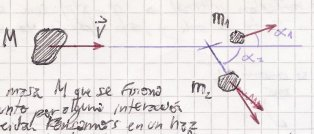
\includegraphics[scale=0.3]{images/fig_mc_dispersion_2cuerpos1.jpg}

Desde el centro de masas se vería una situación como la mostrada en la ilustración

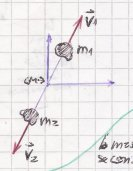
\includegraphics[scale=0.3]{images/fig_mc_dispersion_2cuerpos2.jpg}

La ilustración con coordenadas sería algo como:
\begin{figure}[htb]
	\begin{center}
	\includegraphics[width=0.5\textwidth]{images/fig_mc_disp2body1.pdf}	 
	\end{center}
	\caption{}
\end{figure} 

Desde el centro de masa se conserva el momento, y entonces
\[
	\vb{P}_1 + \vb{P}_2 = 0
\]
\[
	m_1 \vb{v}_1 + m_2 \vb{v}_2 = 0
\]
definimos una velocidad relativa
\[
	\vb{v} \equiv \vb{v}_2  - \vb{v}_1 = \vb{v}_2 \left( \frac{ m_1 + m_2 }{ m_1 }\right) .
\]
\begin{figure}[htb]
	\begin{center}
	\includegraphics[width=0.5\textwidth]{images/fig_mc_disp2body2.pdf}	 
	\end{center}
	\caption{}
\end{figure} 

Con respecto a la energía,
\[
	\frac{1}{2} M \vb{V}_{cm}^2 + e_{int} = \frac{1}{2} m_1 \vb{v}_1^2 + \frac{1}{2} m_2 \vb{v}_2^2
						+ e_{int 1 } + e_{int 2} + \frac{1}{2} M \vb{V}_{cm}^2
\]
\[
	\frac{1}{2} m_1 \vb{v}_1^2 + \frac{1}{2} m_2 \vb{v}_2^2 = e_{int} - e_{int 1 } - e_{int 2} = \Delta e
\]
y pasando todo en términos de la velocidad relativa
\[
	 \frac{1}{2} \frac{m_1 m_2}{ m_1 + m_2 } v = \Delta e
\]
entonces 
\[
	v = \sqrt{\frac{ 2 \Delta e}{ \mu } }.
\]

Como la velocidad relativa $v$ es una constante se sigue que la separación de los cuerpos es a
velocidad constante.
Por otra parte, la energía interna $e$ es la que provoca la fisión. Se puede pensar que existe un
resorte que {\it revienta} espontáneamente y separa ambas partículas.

\begin{figure}[htb]
	\begin{center}
	\includegraphics[width=0.5\textwidth]{images/fig_mc_disp2body3.pdf}	 
	\end{center}
	\caption{}
\end{figure} 

Conocemos el módulo de la velocidad pero no su dirección.
El problema es evidentemente plano. Consideramos que todo se mide desde el centro de masas y el
problema es no relativista.
Desde un sistema laboratorio 
\[
	\vb{V}_1^L =  \vb{V}_{cm} + \vb{V}_1' \qquad \longrightarrow \quad ( \vb{V}_1^L - \vb{V}_{cm} ) = \vb{V}_1'
\]
\[
	{V_1^L}^2 - V_{cm} - 2 {\vb{V}_1^L}^2 \vb{V}_{cm} = V_1^2
\]
\[
	{V_{1x}^L}^2 + {V_{1y}^L}^2 - V_{cm} - 2 {V_{1x}^L}^2 V_{cm} = V_1^2
\]
\[
	( V_{1x}^L  - V_{cm} )^2 + {V_{1y}^L}^2 = V_1^2
\]
que es una circunferencia en el plano.
De la ilustración puede verse que 
\[
	\tan(\theta) = \frac{V_1 \sin(\chi) }{ V_{cm} + V_1 \cos(\chi) }
\]
\begin{figure}[htb]
	\begin{center}
	\includegraphics[width=0.45\textwidth]{images/fig_mc_disp2body4a.pdf}	 
	\includegraphics[width=0.45\textwidth]{images/fig_mc_disp2body4b.pdf}
	\end{center}
	\caption{}
\end{figure} 

Luego, se puede despejar de la anterior ecuación el valor de $\chi$. Para ello se elevan
ambos miembros al cuadrado, se expande como 
\[
	\tan^2 \theta \left( \frac{V_{cm}}{v_1} \right)^2 +
	\tan^2 \theta \cos^2 \chi + 2 \tan \theta \frac{V_{cm}}{v_1} \cos \chi = 1 - \cos^2 \chi
\]
y luego del álgebra resulta 
\[
	\cos \chi = - \sin^2 \theta \pm \frac{2}{1+\tan^2\theta} 
	\sqrt{ 1 + \tan^2 \theta - \tan^2 \theta \left( \frac{V_{cm}}{v_1} \right)^2 }.
\]

Esto tiene dos raíces $\chi_{1,2}$ si $ V_{cm} > V_1$. A un mismo $\theta$ tengo dos $\chi$, uno
correspondiente a partículas rápidas y otro para lentas.

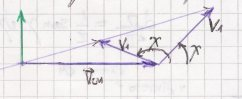
\includegraphics[scale=0.3]{images/fig_mc_dispersion_doschi.jpg}

Hay una $v_1$ para la cual se anula el término dentro de la raíz, que es 
\[
	1 + \tan^2\theta( 1 - \left( \frac{V_{cm}}{V_1} \right)^2 )
\]
y cuando eso sucede se tiene $ V_1 = V_{cm} \sin \theta $.
si $ V_{cm} > V_1$ no hay partículas emitidas hacia atrás,

\includegraphics[scale=0.3]{images/fig_mc_dispersion_caso1.jpg}

a medida que aumenta $\theta$ las partículas lentas y rápidas tendrán velocidades parecidas. Cuando
vale $\theta_t$ no tengo más que una sola velocidad. Para $\theta > \theta_t $ no hay emisión de
partículas.

Si $ V_{cm} > V_1$ hay una sola $V$ de las partículas.

Si $ V_{cm} < V_1$ hay partículas emitidas hacia atrás vistas desde L.

Si pensamos en una distribución isótropa de partículas, desde el centro de masa será proporcional
al ángulo sólido
\[
	\text{ Distribución } \sim d\Omega = 2\pi\sin \chi d\chi,
\]
y entonces el cociente entre la fracción de ángulo de la distribución y el ángulo sólido total,
\[
	\frac{d\Omega}{4\pi} = \frac{1}{2} \sin \chi d\chi.
\]

Podemos evaluar la distribución de energía de las partículas. Desde el centro de masa,
\[
	e = \frac{1}{2} m_1 V_{1}^2
\]
\notamargen{Tenía el comentario: todas las partículas de la fisión tienen igual energía.}
y entonces
\[
	V_L^2 = V_1^2 + V_{cm}^2 - 2 V_1 V_{cm} \cos( \pi -\chi )
\]
a iguales $V_1,V_{cm}$ se tienen variables $V_L, \chi$, entonces
\[
	dV_L^2 = - 2 V_1 V_{cm} \sin(\chi) d\chi
\]
\[
	\frac{dV_L^2}{2 V_1 V_{cm}} = \sin( \chi) d\chi 
\]
\[
	d\sigma = 2 \pi \rho |\dtot{\rho}{\chi}| d\chi 
\]
\[
	d\Omega = 2 \pi \sin( \chi ) d\chi 
\]
\[
	\frac{d\Omega}{4\pi} = \frac{1}{2} \sin( \chi ) d\chi 
\]
\[
	\frac{d\Omega}{4\pi} =  \frac{d (V_L^2) }{4 V_1 V_{cm}} = \frac{1}{2} \frac{d ( 1/2 m_1 V_L^2) }{m_1 V_1 V_{cm}} 
\]

Como la anterior se puede escribir,
\[
	\frac{dT}{2 m_1 V_{cm} v_1}
\]
se ve que representa la fraccióon de partículas entre $T$ y $T+dT$ vistas desde el laboratorio.

Las diferencias entre las distribuciones son patentes en este gráfico:

\includegraphics[scale=0.4]{images/fig_mc_dispersion_distribuciones.jpg}

% =================================================================================================
\section{Scattering}
% =================================================================================================

Tenemos dos suposiciones básicas:
	\begin{itemize}
		\item Interacción elástica.
		\item Conservación de energía y de momento.
	\end{itemize}

\begin{figure}[htb]
	\begin{center}
	\includegraphics[width=0.5\textwidth]{images/fig_mc_scatt1.pdf}	 
	\end{center}
	\caption{}
\end{figure} 	
	
Desde el centro de masa se tienen:
\[
	\vb{P} = \vb{P}_1 + \vb{P}_2 = 0	\qquad		\vb{r} \equiv \vb{r}_2 + \vb{r}_1
	\qquad		\vb{V} \equiv \vb{V}_2 - \vb{V}_1
\]
donde los últimos son las posiciones y velocidades relativas.
\[
	E = \frac{1}{2} M \vb{V}_{cm}^2 + \frac{1}{2} \mu \vb{V}^2 + V(r)
\]
\[
	m_1 \vb{V}_1 + m_2 \vb{V}_2 = 0 \qquad m_1 \vb{V}_1 = -\frac{m_2}{m_1} \vb{V}_2.
\]
\begin{figure}[htb]
	\begin{center}
	\includegraphics[width=0.7\textwidth]{images/fig_mc_scatt2.pdf}	 
	\end{center}
	\caption{}
\end{figure} 
En términos de las velocidades relativas
\[
	\vb{V}_2 = \frac{m_1}{m_1 + m_2} \vb{V} \qquad \vb{V}_1 = -\frac{m_2}{m_1 + m_2} \vb{V}
\]
Se puede escribir la energía cinética del siguiente modo
\[
	T = \frac{1}{2} m_1 \vb{V}_{1-in}^2 + \frac{1}{2} m_2 \vb{V}_{2-in}^2 =
	\frac{1}{2} M \vb{V}_{cm}^2 + \frac{1}{2} m_1 \vb{V}_{1-cm}^2 + \frac{1}{2} m_2 \vb{V}_{2-cm}^2 
\]
\[
	T - \frac{1}{2} M \vb{V}_{cm}^2 \equiv t = \frac{1}{2} \frac{m_1 m_2}{m_1 + m_2} \vb{V}^2 =
							\frac{1}{2} \mu \vb{V}^2
\]

\[
	\vb{V}_1^L = \vb{V}_{cm} - \frac{m_2}{M} \vb{V}	\qquad \vb{V}_2^L = \vb{V}_{cm} - \frac{m_1}{M} \vb{V}
\]

\[
	\vb{p}_1^L = m_1 \vb{V}_{cm} - \mu \vb{V} = m_1 \frac{\vb{P}}{M} - \mu \vb{V}
\]
\[
	\vb{p}_2^L = m_2 \vb{V}_{cm} + \mu \vb{V} = m_2 \frac{\vb{P}}{M} + \mu \vb{V}
\]
\begin{figure}[htb]
	\begin{center}
	\includegraphics[width=0.35\textwidth]{images/fig_mc_scatttriangle.pdf}	 
	\end{center}
	\caption{}
\end{figure} 
Donde 
\[
	\vb{V}_{cm} + \vb{V}_1 = \vb{V}_1^L
\]
\[
	\vb{p}_2^L = \frac{m_2}{M} \vb{P} + \mu \vb{V}\hat{n}		\qquad	 \vb{p}_1^L = \frac{m_1}{M} \vb{P} - \mu \vb{V}\hat{n}
\]
\[
	\frac{m_2}{M} \vb{P} + \frac{m_1}{M} \vb{P} = \vb{P} = \vb{p}_2^L + \vb{p}_1^L
\]
\[
	\tan(\theta_2) = \frac{P_1 \sin(\chi)}{ (m_2/M) P + P_1\cos(\chi)}
\]

% =================================================================================================
\section{Dispersión por potenciales infinitos}
% =================================================================================================

La idea es que sabiendo $\rho$ (parámetro de impacto) quiero saber qué ángulo $\chi$ se desvían las
partículas incidentes.
\begin{figure}[htb]
	\begin{center}
	\includegraphics[width=0.7\textwidth]{images/fig_mc_potinf.pdf}	 
	\end{center}
	\caption{}
\end{figure} 
\[
	\phi_0 + \alpha = \frac{\pi}{2}		\qquad		2 \phi_0 + \alpha + \beta = \pi
	\qquad \phi_0 + \beta = \frac{\pi}{2}
\]
\[
	\alpha = \beta		\qquad 		2\alpha = 2\beta = \chi
\]
\[
	\dtot{\rho}{z} = \tan \left(\beta \right) = \tan\left(\frac{\chi}{2}\right)
\]
\[
	\tan\left(\frac{\chi}{2}\right) = \dtot{\rho}{z} = \frac{ d\rho/dz }{ dz/d\theta }
\]
con $\theta$ variable paramétrica. Donde $\rho = \rho(z)$ es la función que da la curva roja (el perfil
del cuerpo dispersor).



% =================================================================================================

% \bibliographystyle{CBFT-apa-good}	% (uses file "apa-good.bst")
% \bibliography{CBFT.Referencias} % La base de datos bibliográfica

\end{document}
